\resizebox{\textwidth}{!}{%
\begin{tikzpicture}[x=1mm,y=1mm, every node/.append style={execute at begin node={\hyphenpenalty=10000\exhyphenpenalty=10000}}]
% phase bands (x is piecewise: Jan-Aug compressed, October expanded; breaks drawn on the axis)
\fill[band] (-1,-31) rectangle (34,25);
\fill[band!55] (34.6,-31) rectangle (60,25);
\fill[band] (60.6,-31) rectangle (121,25);
\fill[band!55] (121.6,-31) rectangle (149,25);
\foreach \x/\t in {16.5/Foundation, 47.3/Product, 90.8/Detection, 135.3/Material}
  \node[font=\scshape\fontsize{6.6}{7}\selectfont, color=mute] at (\x,22.8) {\t};
% axis
\draw[ink, line width=0.4pt] (-1,0) -- (149,0);
\foreach \x/\d in {0/Jan,10/Mar,20/Apr,30/May,36/Jul,48/Aug,62/14 Oct,80/19 Oct,98/22 Oct,112/29 Oct,128/31 Oct,146/1 Nov}
  {\draw[ink] (\x,0) -- (\x,-0.9); \node[font=\fontsize{5.6}{6}\selectfont, color=mute, below] at (\x,-0.9) {\d};}
\foreach \b in {34.3,60.3} {\fill[band] (\b-0.9,-1.2) rectangle (\b+0.9,1.2);
  \draw[ink] (\b-1.4,-1.2) -- (\b-0.4,1.2); \draw[ink] (\b+0.4,-1.2) -- (\b+1.4,1.2);}
% milestones (above)
\foreach \x/\h/\w/\t in {
 {0/12/17mm/{\textbf{26 Jan} first\\commit: HE5 and\\TIF readers}},
 {10/4/9mm/{\textbf{23 Mar}\\first\\trainer}},
 {20/12/13mm/{\textbf{10 Apr}\\hyperspectral\\SegFormer MAE}},
 {36/4/22mm/{\textbf{23 Jul} backend +\\frontend: the app}},
 {62/12/17mm/{\textbf{14 Oct} Spectral-\\Earth pretraining,\\wavelength stem}},
 {66/3/13mm/{\textbf{15 Oct}\\residual\\Mahalanobis}},
 {80/12/17mm/{\textbf{19 Oct} FT04\\ships as V2,\\pAUC 0.170}},
 {106/12/18mm/{\textbf{28--29 Oct}\\Heavy on an H100:\\0.189, v2.1.0}},
 {128/12/13mm/{\textbf{31 Oct}\\namer N001b\\passes level 1}}}
 {\draw[ink, line width=0.35pt] (\x,0) -- (\x,\h); \fill[ink] (\x,0) circle (0.7); \node[ms=\w] at (\x+0.6,\h-0.6) {\t};}
\draw[ochre, line width=0.6pt] (146,0) -- (146,4); \fill[ochre] (146,0) circle (1.1);
\node[font=\fontsize{7}{8}\selectfont, anchor=south east, align=right] at (148,4.3) {\textbf{v1.0}};
% failures (below): x, level, width, text
\foreach \x/\h/\w/\t in {
 {30/-5/17mm/{\textbf{May} plain RX\\fails: covariance\\near singular,\\distances $10^{11}$\\$\to$ MNF-RX}},
 {48/-5/12.5mm/{\textbf{Aug} two\\outages hit\\main; fake\\docs removed\\$\to$ check\\the worker}},
 {98/-5/13mm/{\textbf{22 Oct} FT07,\\FT08: 0.165,\\0.164 $<$ 0.170\\$\to$ widen\\the model}},
 {112/-5/11mm/{\textbf{29 Oct}\\haze read\\as cloud:\\209 of 230\\targets $\to$\\thick only}},
 {124/-17/13mm/{\textbf{31 Oct}\\HyperSL:\\0.083 $<$ 0.128\\$\to$ rejected}},
 {130/-5/13mm/{\textbf{31 Oct}\\N001 level 1\\at chance\\(0.50) $\to$\\matching}}}
 {\draw[manmade!60, line width=0.35pt] (\x,-3.3) -- (\x,\h); \draw[manmade, line width=0.5pt] (\x-0.7,-0.7) -- (\x+0.7,0.7) (\x-0.7,0.7) -- (\x+0.7,-0.7); \node[fl=\w] at (\x+0.6,\h+0.6) {\t};}
\draw[manmade!60, line width=0.35pt] (146,-3.3) -- (146,-17);
\draw[manmade, line width=0.5pt] (145.3,-0.7) -- (146.7,0.7) (145.3,0.7) -- (146.7,-0.7);
\node[fl=10mm, anchor=north east, align=right] at (147.5,-17.6) {\textbf{1 Nov}\\PV spectra:\\no effect};
% pAUC sparkline (matplotlib, figures/chart_spark.pdf)
\node[anchor=south west, inner sep=0] at (63,-30) {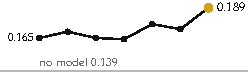
\includegraphics[width=42mm]{figures/chart_spark.pdf}};
\node[font=\fontsize{5.6}{6}\selectfont, color=mute, anchor=north west] at (64,-30.3) {pAUC: v0.2.0, FT04, FT07, FT08, FT09b, FT09c, Heavy};
\end{tikzpicture}}
